\subsection{Booking page}
The booking procedure is held through six steps divided into two pages. 
\par \noindent In the first page there are three subsections: the first one is used to decide the date of arrival and departure with a possibility to add some requests in the specific window, the second one is used to select the number of rooms and guests, the third subsection is reserved to the selection of the room, presented as a carousel with the type and the description of each room, it is possible to use the "prev" and "next" button to navigate the carousel.
\par \noindent The second page displays three steps to complete the booking. The first section is dedicated to the insert guest information, some of the fields i.e. phone number and email are requested only for people over age of 18. It is possible to add different guests by using the plus button. The next section shows the summary of the booking with all the details and the last one directs to the payment. 

\begin{figure}[H]
	\centering
	%\label{fig:manager-index}
	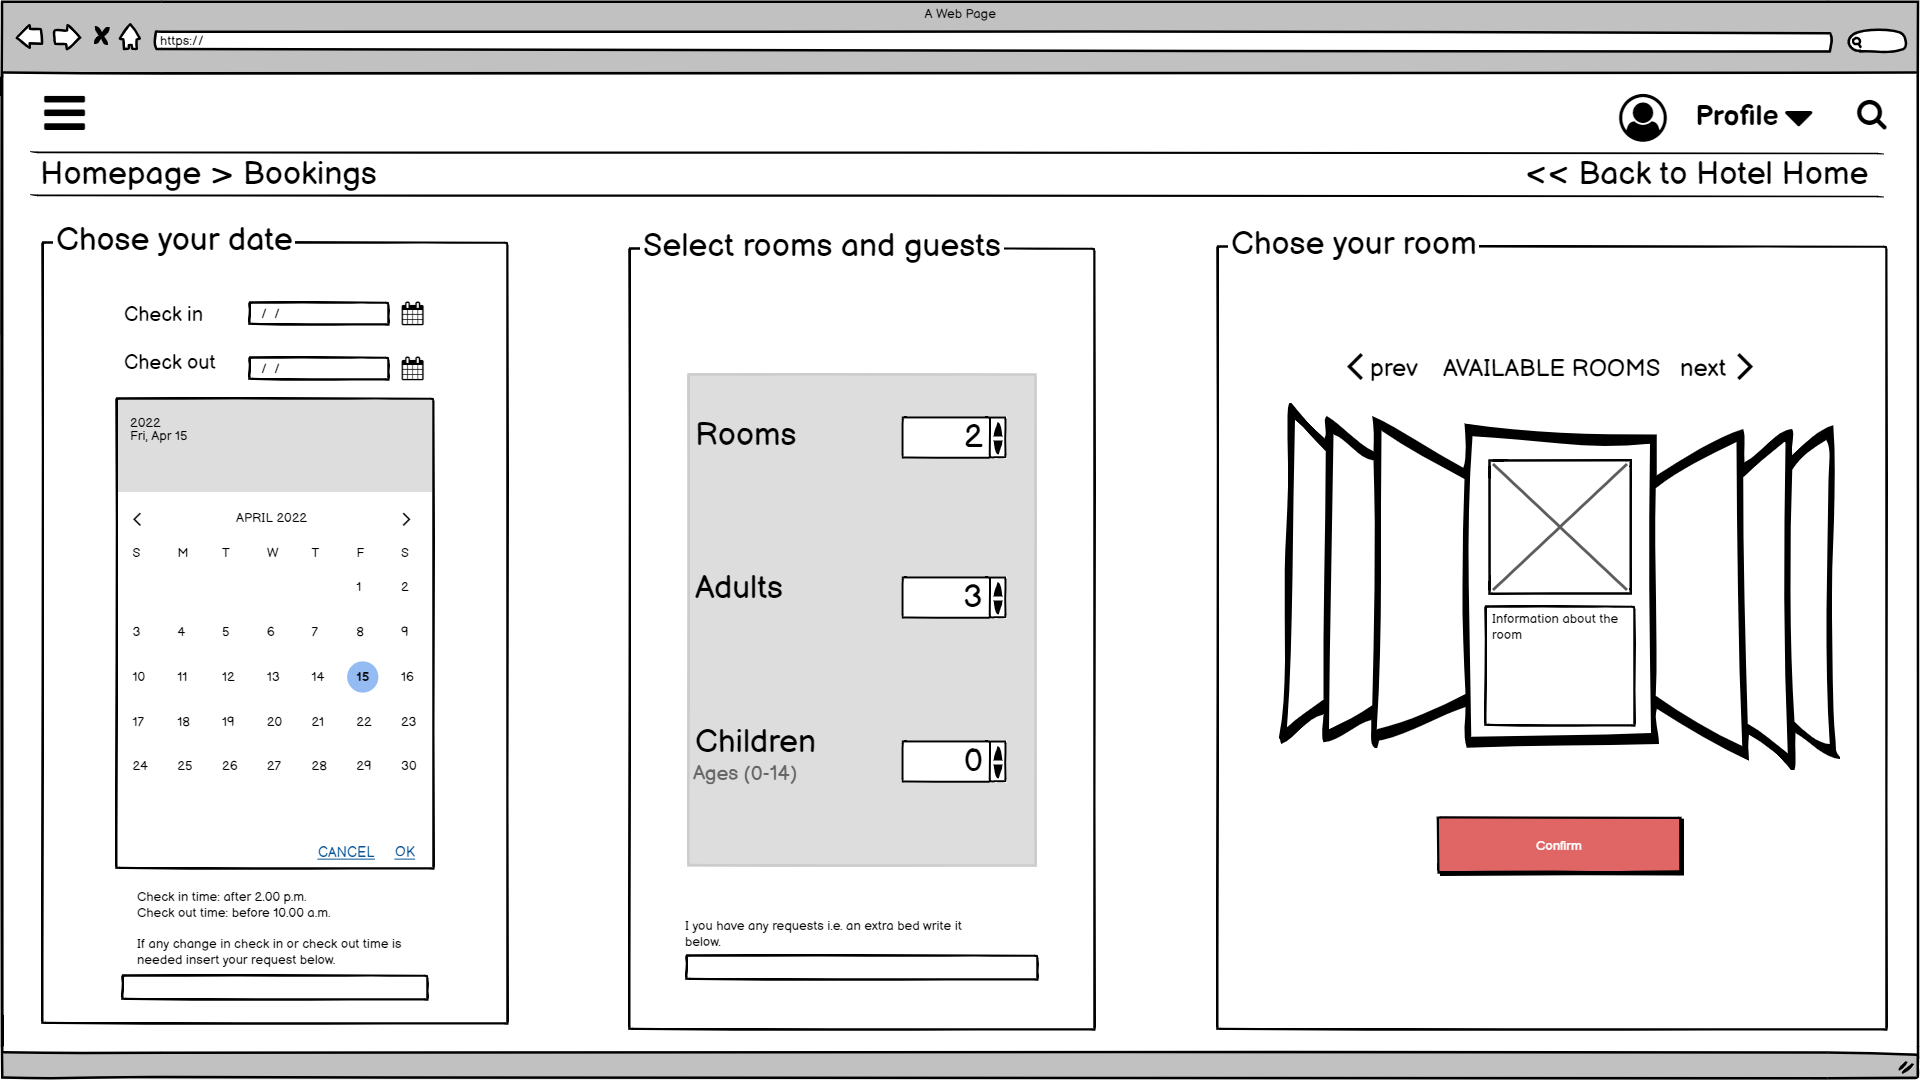
\includegraphics[height=7.5cm]{images/Booking.png} 
	\caption{Booking pages: first page}
\end{figure}
\begin{figure}[H]
	\centering
	%\label{fig:manager-index}
	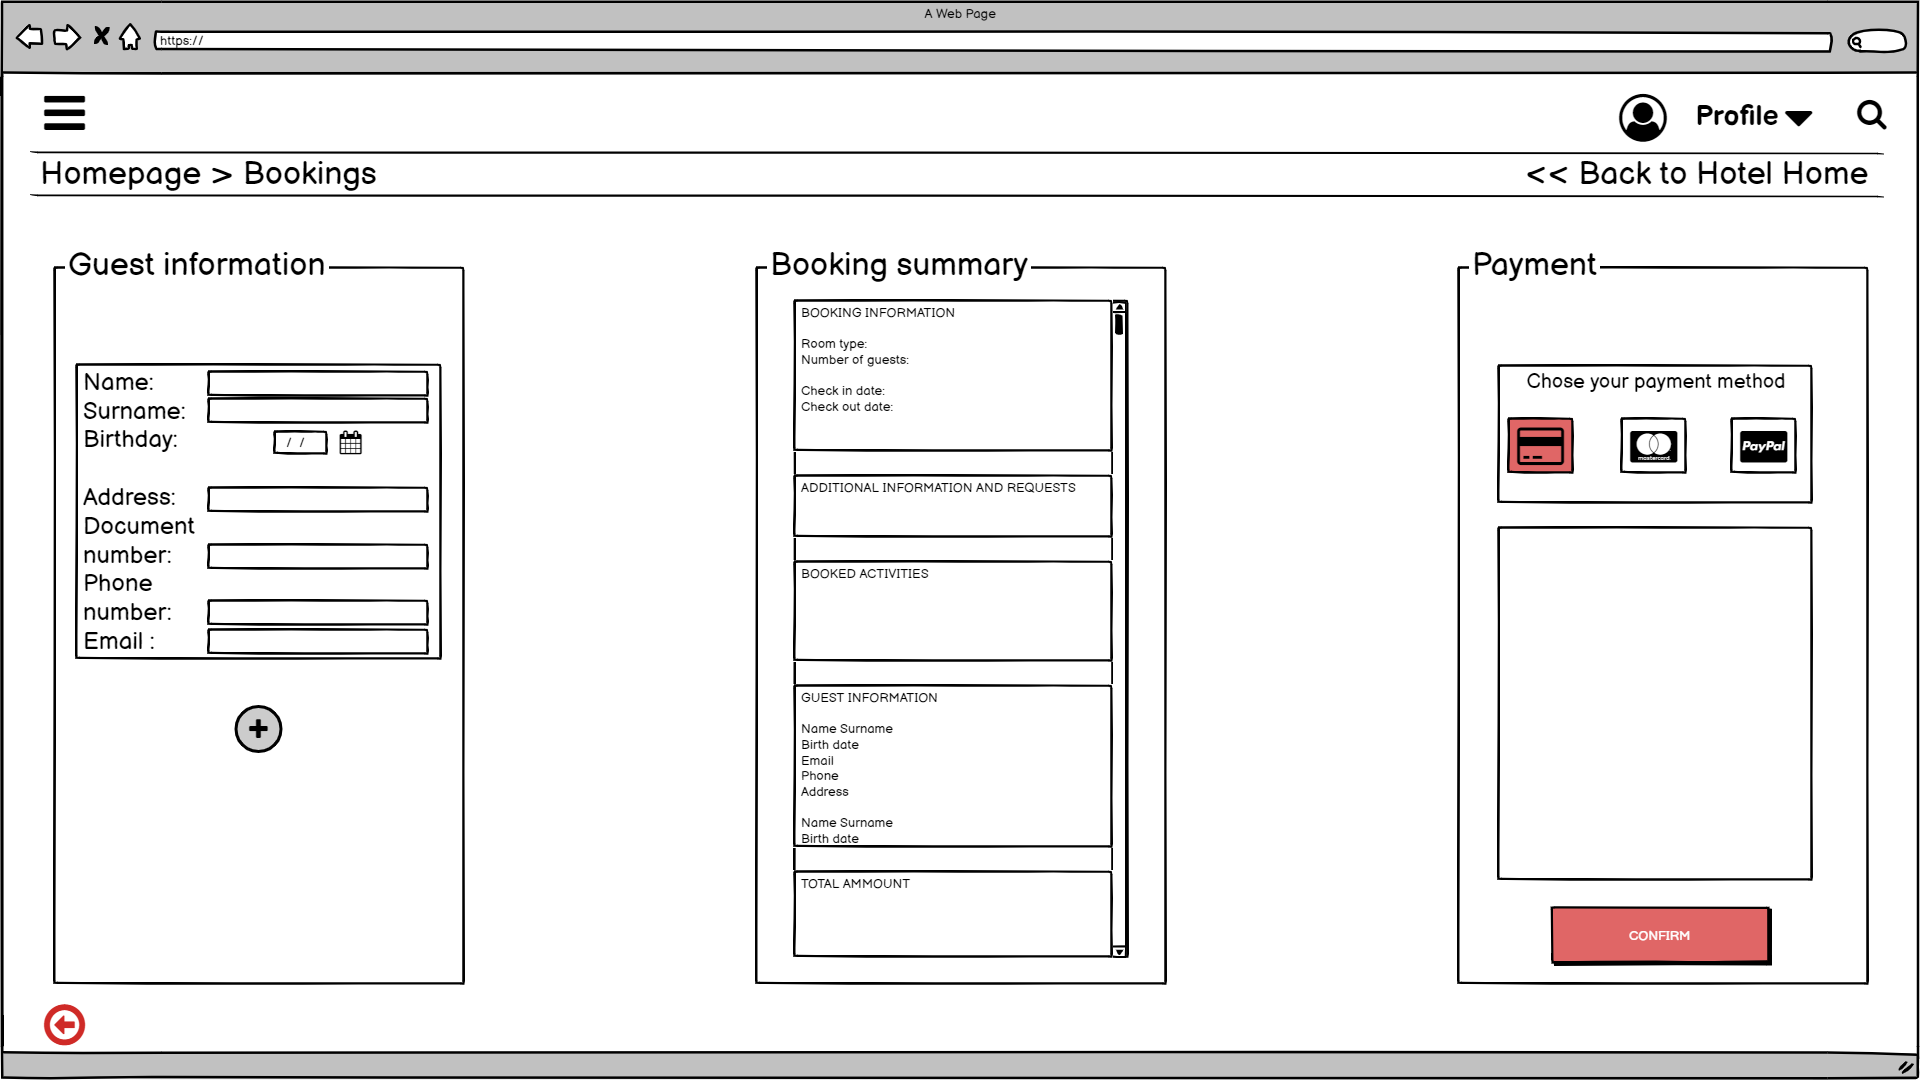
\includegraphics[height=7.5cm]{images/booking_2.png} 
	\caption{Booking pages: second page}
\end{figure}